% This LaTeX was auto-generated from MATLAB code.
% To make changes, update the MATLAB code and export to LaTeX again.

\documentclass{article}

\usepackage[utf8]{inputenc}
\usepackage[T1]{fontenc}
\usepackage{lmodern}
\usepackage{graphicx}
\usepackage{color}
\usepackage{hyperref}
\usepackage{amsmath}
\usepackage{amsfonts}
\usepackage{epstopdf}
\usepackage[table]{xcolor}
\usepackage{matlab}

\sloppy
\epstopdfsetup{outdir=./}
\graphicspath{ {./HW9_code_images/} }

\matlabhastoc

\matlabmultipletitles

\begin{document}

\maketitle
\thispagestyle{empty}
\pagebreak
\matlabtableofcontents{Table of Contents}

\begin{par}
\begin{flushleft}
In this homework assignment, an autoencoder with different number of unit in its hidden layer is trained and evaluated on MNIST handwritten digit dataset.
\end{flushleft}
\end{par}

\begin{matlabcode}
clc; clear; close all;
load('HW9_code_workspace.mat');
\end{matlabcode}
\pagebreak

\label{T_AF22880B}
\matlabtitle{0. MNIST Dataset}

\label{H_FBA02D0E}
\matlabheading{0.1 Downloading MNIST Dataset and Import into \textit{Matlab}}

\begin{par}
\begin{flushleft}
The code snippet below will download MNIST dataset from web and extract the downloaded file into Matlab matrices as test and train images and labels.
\end{flushleft}
\end{par}

\begin{matlabcode}
mnist_train_image = 'train-images-idx3-ubyte';
mnist_train_label = 'train-labels-idx1-ubyte';
mnist_test_image  = 't10k-images-idx3-ubyte';
mnist_test_label  = 't10k-labels-idx1-ubyte';
train_set_number  = 60000;
test_set_number   = 10000;

downloadMNIST(mnist_train_image, mnist_train_label, mnist_test_image, mnist_test_label);
\end{matlabcode}
\begin{matlaboutput}
MNIST dataset already downloaded.
\end{matlaboutput}


\begin{matlabcode}
[train_images, train_labels] = readMNIST(mnist_train_image, mnist_train_label, train_set_number);
[test_images,   test_labels] = readMNIST(mnist_test_image, mnist_test_label, test_set_number);

clear mnist_train_image mnist_train_label mnist_test_image mnist_test_label train_set_number test_set_number
\end{matlabcode}


\label{H_3C76610B}
\matlabheading{0.2 Plotting a Sample of MNIST Dataset}

\begin{par}
\begin{flushleft}
A set of 100 randomly chosen samples of the training dataset is plotted here.
\end{flushleft}
\end{par}

\begin{matlabcode}
random_indices = randi(60000, [1 100]);
montage(train_images(:, :, random_indices), 'BorderSize', [2 2], 'BackgroundColor', 'white');
\end{matlabcode}
\begin{center}
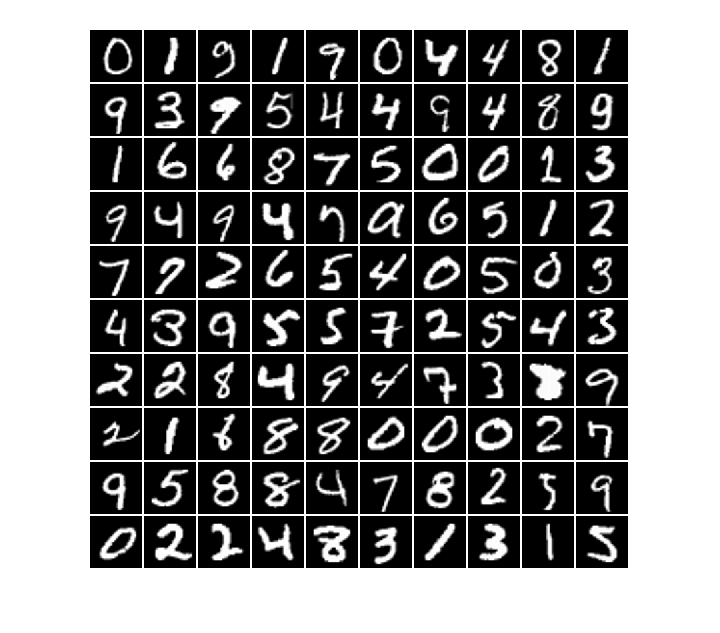
\includegraphics[width=\maxwidth{72.25288509784245em}]{figure_0.png}
\end{center}
\pagebreak

\label{T_66B21DAF}
\matlabtitle{1. 3-Layer Autoencoder with Different Hidden Units}

\begin{par}
\begin{flushleft}
In this section we train an autoencoder with 5, 10, 30 and 60 units in its hidden layer.
\end{flushleft}
\end{par}

\label{H_257D6130}
\matlabheading{1.1 Reshapinng the Images}

\begin{par}
\begin{flushleft}
To train the network, we reshape the 28x28 images to vectors of 784 element, to feed them into the input layer with the same number of units (784). 
\end{flushleft}
\end{par}

\begin{matlabcode}
train_images_reshaped = reshape(train_images, [size(train_images, 1)*size(train_images, 2) size(train_images, 3)]);
test_images_reshaped  = reshape(test_images,  [size(test_images, 1)*size(test_images, 2) size(test_images, 3)]);
\end{matlabcode}


\begin{par}
\begin{flushleft}
We also sampled 16 images of the test dataset to check the reconstruction performance of each autoencoder visually.
\end{flushleft}
\end{par}

\begin{matlabcode}
sample_original_images  = train_images_reshaped(:, [11 3 2 33 5 24 22 1 85 13 100:105]);
\end{matlabcode}
\pagebreak

\label{H_6BC5880B}
\matlabheading{1.2 Autoencoder with 5 Hidden Units}

\begin{par}
\begin{flushleft}
We trained a 3-layer autoencoder with a hidden layer consisting of 5 hidden units. The learning curve is plotted below.
\end{flushleft}
\end{par}

\begin{matlabcode}
autoenc_5 = trainAutoencoder(train_images_reshaped, 5, ...
                            'MaxEpochs', 400, ...
                            'L2WeightRegularization', 0.004, ...
                            'SparsityRegularization', 4, ...
                            'SparsityProportion', 0.15);
\end{matlabcode}

\begin{par}
\begin{flushleft}
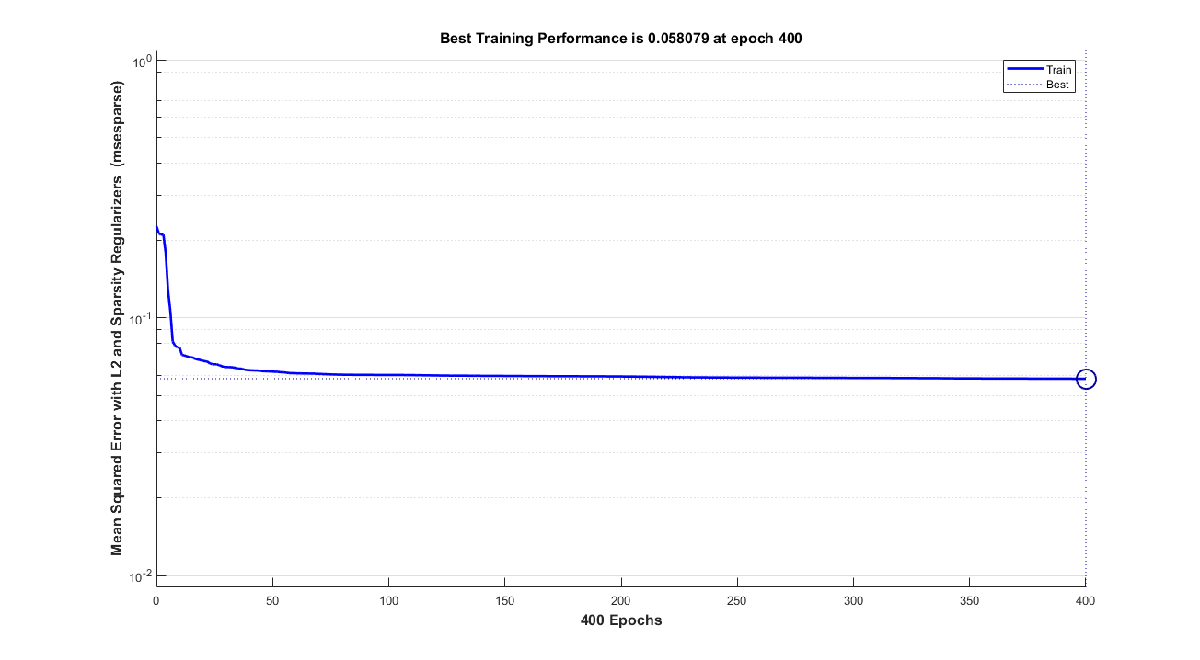
\includegraphics[width=\maxwidth{86.10737802033681em}]{image_0}
\end{flushleft}
\end{par}


\begin{par}
\begin{flushleft}
To view the structure of the network we can get help from built-in functions of Matlab. 
\end{flushleft}
\end{par}

\begin{matlabcode}
view(autoenc_5);
\end{matlabcode}

\begin{par}
\begin{flushleft}
\centering
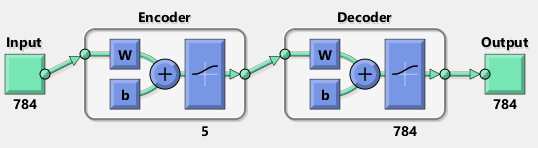
\includegraphics[scale=0.5]{image_1}
\end{flushleft}
\end{par}


\begin{par}
\begin{flushleft}
16 sample of the test images (which were never presented to the autoencoder in training process)  are chosen to feed the autoencoder so we can visually evaluate the reconstruction performance of the trained autoencoder.
\end{flushleft}
\end{par}

\begin{matlabcode}
reconstructed_images_5  = predict(autoenc_5 , sample_original_images);
display_original_images_vs_reconstructed(sample_original_images, reconstructed_images_5);
\end{matlabcode}
\begin{center}
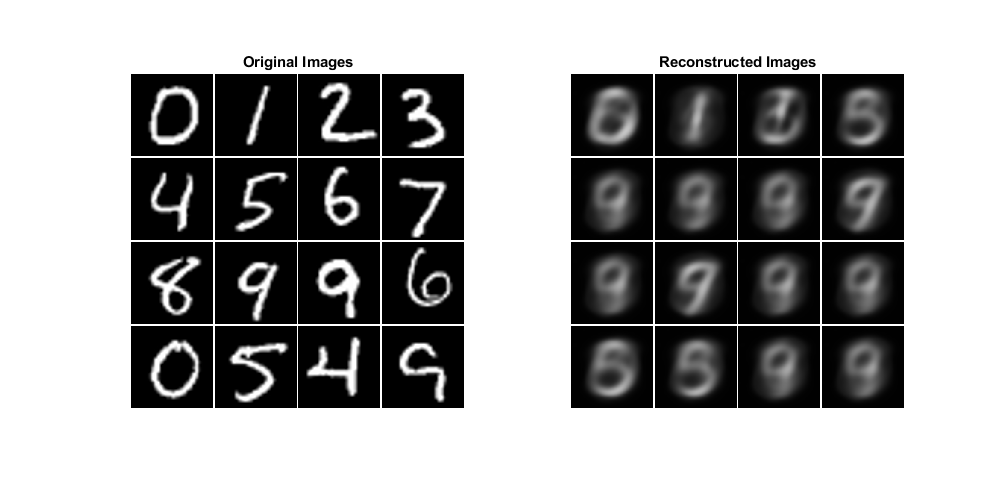
\includegraphics[width=\maxwidth{100.35122930255896em}]{figure_1.png}
\end{center}
\pagebreak

\label{H_BD0471C1}
\matlabheading{1.3 Autoencoder with 10 Hidden Units}

\begin{par}
\begin{flushleft}
We trained a 3-layer autoencoder with a hidden layer consisting of 10 hidden units. The learning curve is plotted below.
\end{flushleft}
\end{par}

\begin{matlabcode}
autoenc_10 = trainAutoencoder(train_images_reshaped, 10, ...
                            'MaxEpochs', 400, ...
                            'L2WeightRegularization', 0.004, ...
                            'SparsityRegularization', 4, ...
                            'SparsityProportion', 0.15);
\end{matlabcode}

\begin{par}
\begin{flushleft}
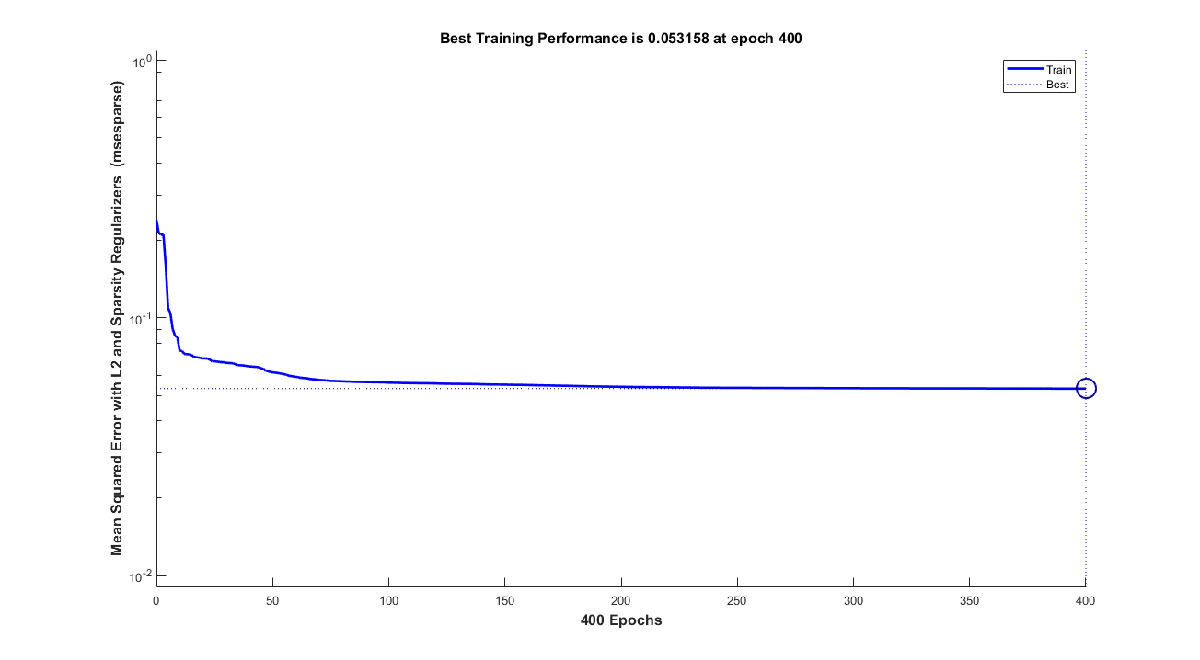
\includegraphics[width=\maxwidth{109.37280481685902em}]{image_2}
\end{flushleft}
\end{par}


\begin{par}
\begin{flushleft}
To view the structure of the network we can get help from built-in functions of Matlab. 
\end{flushleft}
\end{par}

\begin{matlabcode}
view(autoenc_10);
\end{matlabcode}

\begin{par}
\begin{flushleft}
\centering
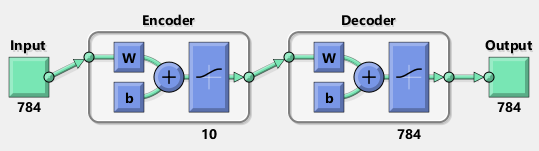
\includegraphics[scale=0.5]{image_3}
\end{flushleft}
\end{par}


\begin{par}
\begin{flushleft}
16 sample of the test images (which were never presented to the autoencoder in training process)  are chosen to feed the autoencoder so we can visually evaluate the reconstruction performance of the trained autoencoder.
\end{flushleft}
\end{par}

\begin{matlabcode}
reconstructed_images_10 = predict(autoenc_10, sample_original_images);
display_original_images_vs_reconstructed(sample_original_images, reconstructed_images_10);
\end{matlabcode}
\begin{center}
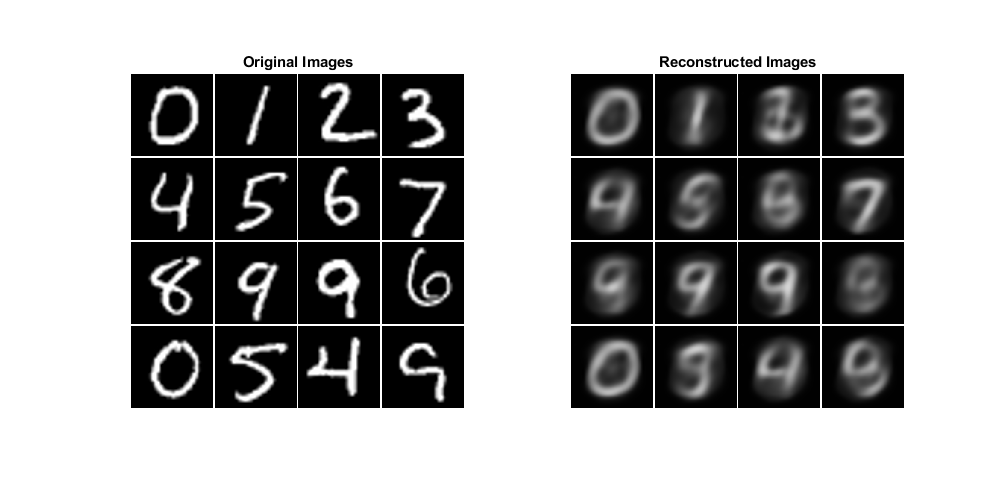
\includegraphics[width=\maxwidth{100.35122930255896em}]{figure_2.png}
\end{center}
\pagebreak

\label{H_D7030029}
\matlabheading{1.4 Autoencoder with 30 Hidden Units}

\begin{par}
\begin{flushleft}
We trained a 3-layer autoencoder with a hidden layer consisting of 30 hidden units. The learning curve is plotted below.
\end{flushleft}
\end{par}

\begin{matlabcode}
autoenc_30 = trainAutoencoder(train_images_reshaped, 30, ...
                            'MaxEpochs', 400, ...
                            'L2WeightRegularization', 0.004, ...
                            'SparsityRegularization', 4, ...
                            'SparsityProportion', 0.15);
\end{matlabcode}

\begin{par}
\begin{flushleft}
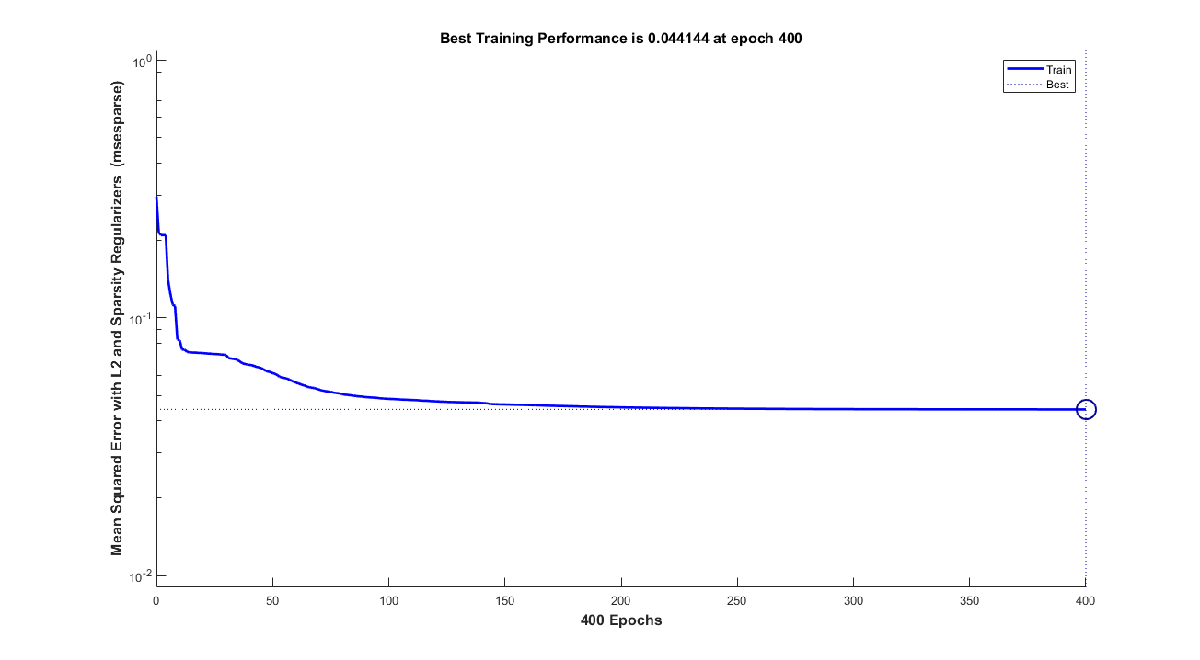
\includegraphics[width=\maxwidth{109.37280481685902em}]{image_4}
\end{flushleft}
\end{par}


\begin{par}
\begin{flushleft}
To view the structure of the network we can get help from built-in functions of Matlab. 
\end{flushleft}
\end{par}

\begin{matlabcode}
view(autoenc_30);
\end{matlabcode}

\begin{par}
\begin{flushleft}
\centering
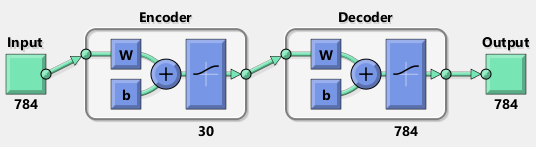
\includegraphics[scale=0.5]{image_5}
\end{flushleft}
\end{par}


\begin{par}
\begin{flushleft}
16 sample of the test images (which were never presented to the autoencoder in training process)  are chosen to feed the autoencoder so we can visually evaluate the reconstruction performance of the trained autoencoder.
\end{flushleft}
\end{par}

\begin{matlabcode}
reconstructed_images_30 = predict(autoenc_30, sample_original_images);
display_original_images_vs_reconstructed(sample_original_images, reconstructed_images_30);
\end{matlabcode}
\begin{center}
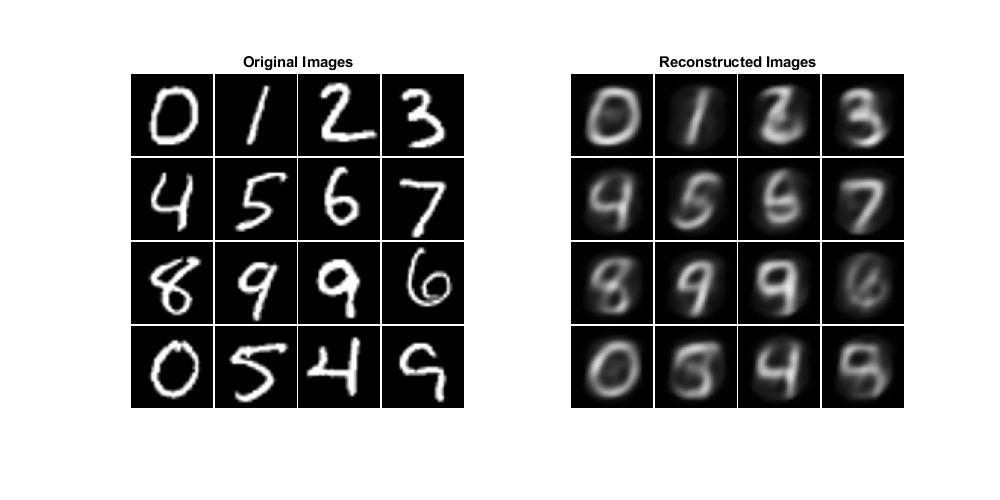
\includegraphics[width=\maxwidth{100.35122930255896em}]{figure_3.png}
\end{center}
\pagebreak

\label{H_F4569F50}
\matlabheading{1.5 Autoencoder with 60 Hidden Units}

\begin{par}
\begin{flushleft}
We trained a 3-layer autoencoder with a hidden layer consisting of 60 hidden units. The learning curve is plotted below.
\end{flushleft}
\end{par}

\begin{matlabcode}
autoenc_60 = trainAutoencoder(train_images_reshaped, 60, ...
                            'MaxEpochs', 400, ...
                            'L2WeightRegularization', 0.004, ...
                            'SparsityRegularization', 4, ...
                            'SparsityProportion', 0.15);
\end{matlabcode}

\begin{par}
\begin{flushleft}
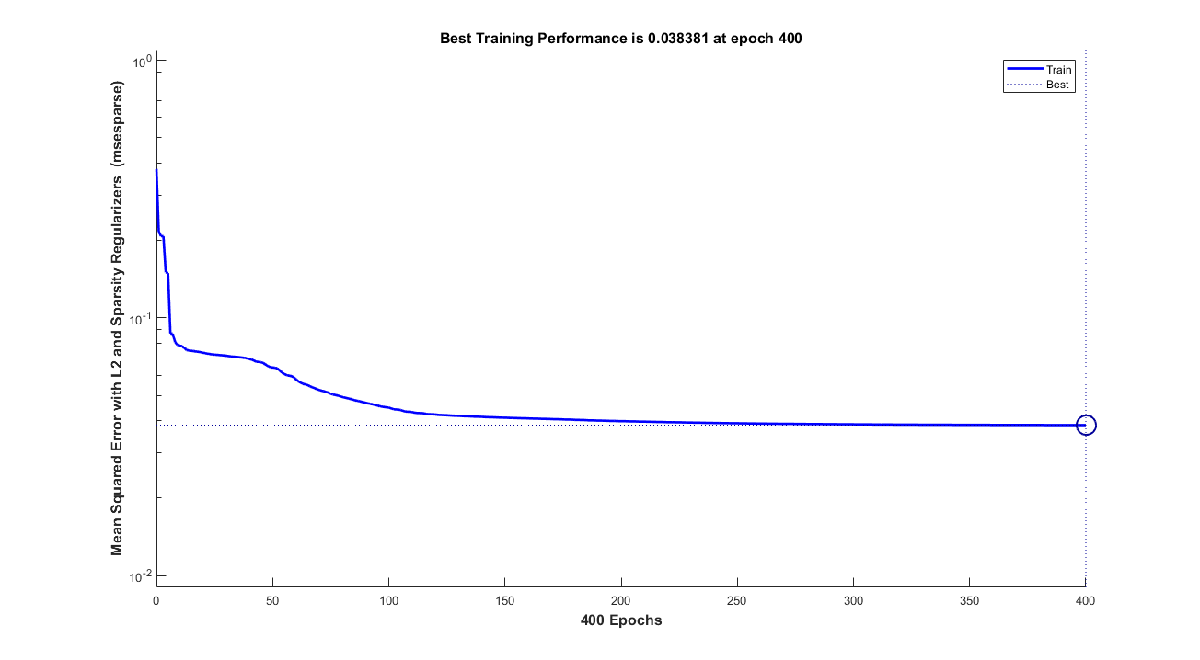
\includegraphics[width=\maxwidth{109.37280481685902em}]{image_6}
\end{flushleft}
\end{par}


\begin{par}
\begin{flushleft}
To view the structure of the network we can get help from built-in functions of Matlab. 
\end{flushleft}
\end{par}

\begin{matlabcode}
view(autoenc_60);
\end{matlabcode}

\begin{par}
\begin{flushleft}
\centering
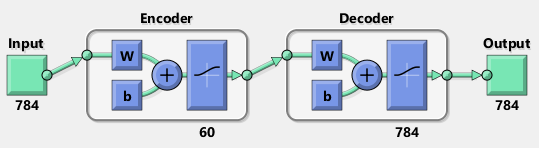
\includegraphics[scale=0.5]{image_7}
\end{flushleft}
\end{par}


\begin{par}
\begin{flushleft}
16 sample of the test images (which were never presented to the autoencoder in training process)  are chosen to feed the autoencoder so we can visually evaluate the reconstruction performance of the trained autoencoder.
\end{flushleft}
\end{par}

\begin{matlabcode}
reconstructed_images_60 = predict(autoenc_60, sample_original_images);
display_original_images_vs_reconstructed(sample_original_images, reconstructed_images_60);
\end{matlabcode}
\begin{center}
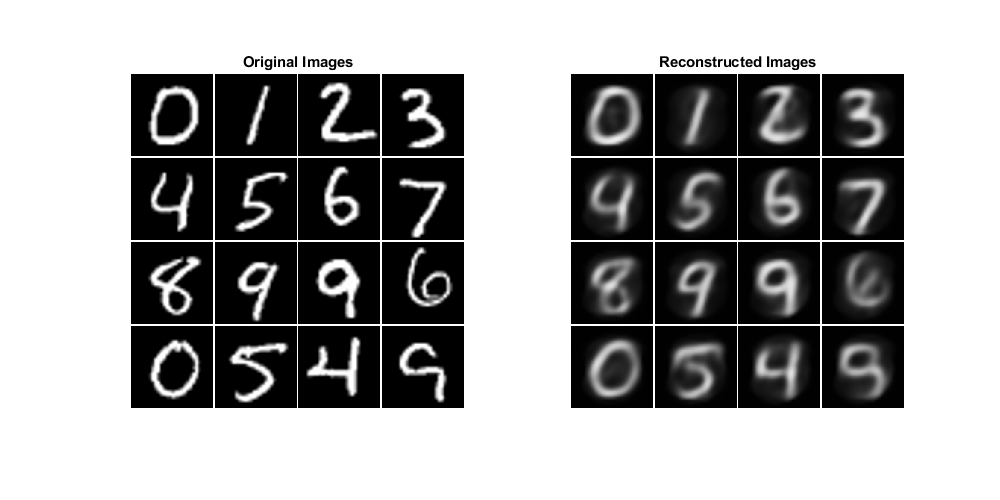
\includegraphics[width=\maxwidth{100.35122930255896em}]{figure_4.png}
\end{center}
\pagebreak

\label{T_DB451F83}
\matlabtitle{2. Display Encoder Weights}

\begin{par}
\begin{flushleft}
In this section, we have plotted the 784 weights of every node in the hidden layer as a 28x28 image.
\end{flushleft}
\end{par}

\label{H_383FBA07}
\matlabheading{2.1 Weights of Autoencoder with 5 Hidden Units}

\begin{matlabcode}
iMontage(autoenc_5.EncoderWeights');
\end{matlabcode}
\begin{center}
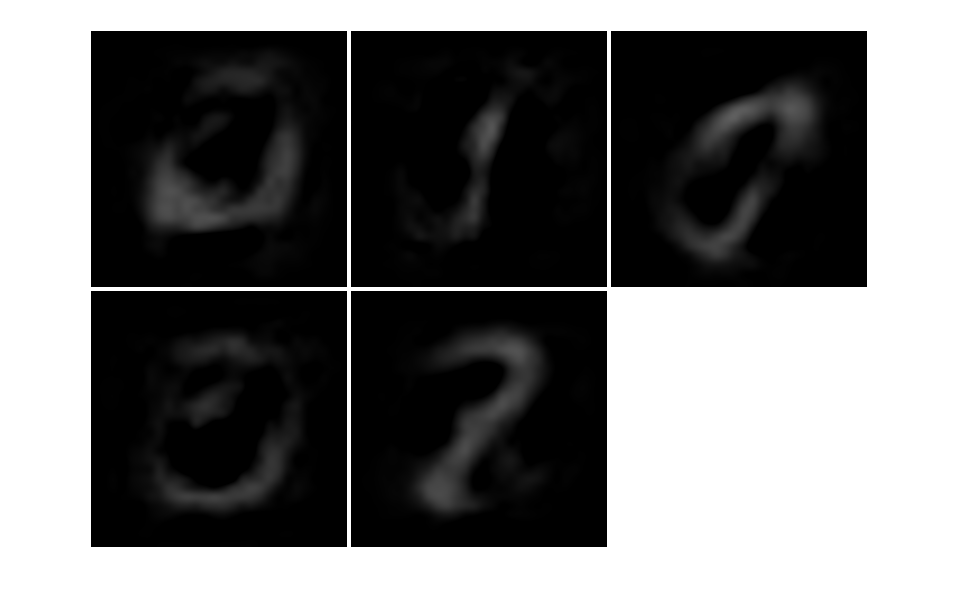
\includegraphics[width=\maxwidth{80.28098344204717em}]{figure_5.png}
\end{center}
\pagebreak

\label{H_12343465}
\matlabheading{2.2 Weights of Autoencoder with 10 Hidden Units}

\begin{matlabcode}
iMontage(autoenc_10.EncoderWeights');
\end{matlabcode}
\begin{center}
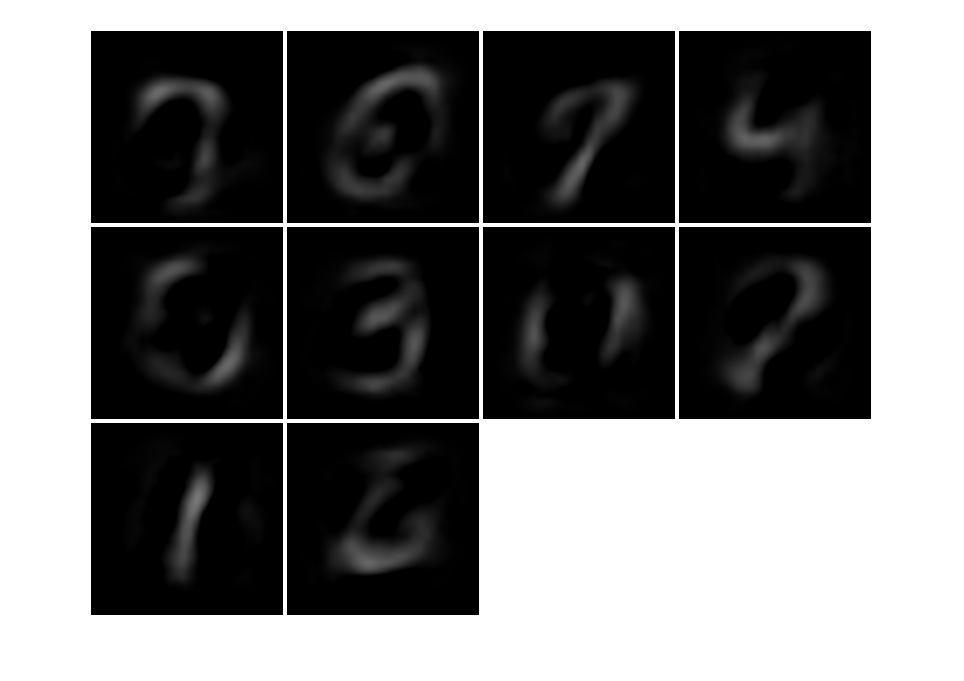
\includegraphics[width=\maxwidth{80.28098344204717em}]{figure_6.png}
\end{center}
\pagebreak

\label{H_551CF159}
\matlabheading{2.3 Weights of Autoencoder with 30 Hidden Units}

\begin{matlabcode}
iMontage(autoenc_30.EncoderWeights');
\end{matlabcode}
\begin{center}
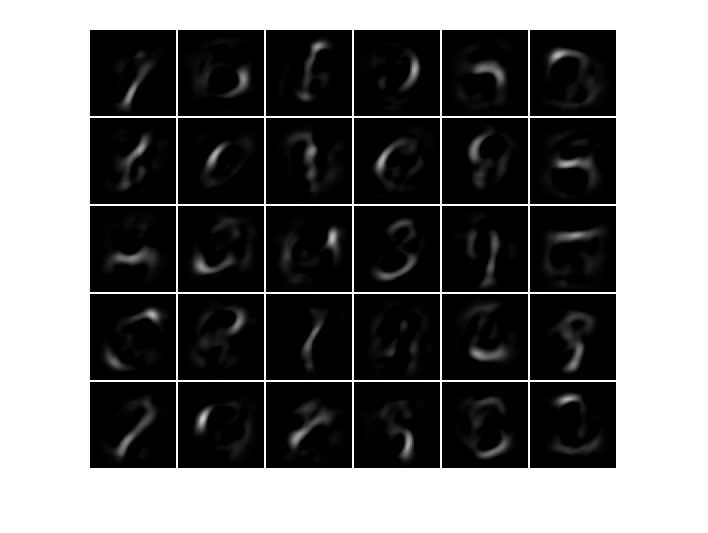
\includegraphics[width=\maxwidth{71.04867034621174em}]{figure_7.png}
\end{center}
\pagebreak

\label{H_F9013831}
\matlabheading{2.4 Weights of Autoencoder with 60 Hidden Units}

\begin{matlabcode}
iMontage(autoenc_60.EncoderWeights');
\end{matlabcode}
\begin{center}
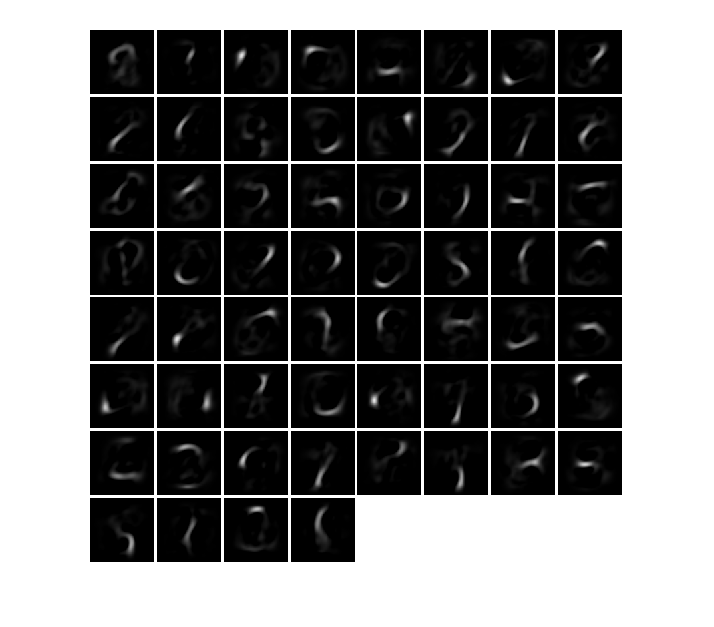
\includegraphics[width=\maxwidth{71.6507777220271em}]{figure_8.png}
\end{center}
\pagebreak

\label{T_335396E5}
\matlabtitle{3. Classifiaction Using Encoded Images}

\begin{par}
\begin{flushleft}
This section will use the encoded version of the images (which are derived from the hidden layer of the autoencoders in the previous section) to classify MNIST dataset.
\end{flushleft}
\end{par}


\label{H_66F4C6C5}
\matlabheading{3.1 One Hot Labels}

\begin{par}
\begin{flushleft}
The 2 line codes below will change the labels into a one-hot-encoded matrix.
\end{flushleft}
\end{par}

\begin{matlabcode}
train_labels_one_hot_encoded = full(ind2vec(train_labels'+1));
test_labels_one_hot_encoded  = full(ind2vec(test_labels'+1));
\end{matlabcode}


\label{H_127F5D6A}
\matlabheading{3.1 Encoded Images}

\begin{par}
\begin{flushleft}
Output of the hidden layer of every autoencoder are stored in the variables \textit{features\_5, features\_10, ..., features\_60.}
\end{flushleft}
\end{par}

\begin{matlabcode}
features_5  = encode(autoenc_5,  train_images_reshaped);
features_10 = encode(autoenc_10, train_images_reshaped);
features_30 = encode(autoenc_30, train_images_reshaped);
features_60 = encode(autoenc_60, train_images_reshaped);
\end{matlabcode}


\label{H_C6A0D472}
\matlabheading{3.2 Softmax Layer}

\begin{par}
\begin{flushleft}
Here we have trained only a softmax layer for classification. The inputs are the features extraced above and the outputs are the labels of evey image.
\end{flushleft}
\end{par}

\begin{matlabcode}
classifier_layer_5  = trainSoftmaxLayer(features_5,  train_labels_one_hot_encoded, 'MaxEpochs', 400);
classifier_layer_10 = trainSoftmaxLayer(features_10, train_labels_one_hot_encoded, 'MaxEpochs', 400);
classifier_layer_30 = trainSoftmaxLayer(features_30, train_labels_one_hot_encoded, 'MaxEpochs', 400);
classifier_layer_60 = trainSoftmaxLayer(features_60, train_labels_one_hot_encoded, 'MaxEpochs', 400);
\end{matlabcode}


\label{H_ABE16252}
\matlabheading{3.3 Classifier Networks}

\begin{par}
\begin{flushleft}
We now attach the trained softmax layer to the output of the hidden layer of the previously trained autoencoders.
\end{flushleft}
\end{par}

\label{H_EE34C0B7}
\matlabheadingtwo{3.3.1 Classifier with 5 Features}

\begin{matlabcode}
stackednet_5 = stack(autoenc_5, classifier_layer_5);
view(stackednet_5);
\end{matlabcode}

\begin{par}
\begin{flushleft}
\centering
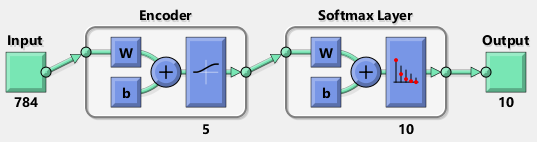
\includegraphics[scale=0.5]{image_8}
\end{flushleft}
\end{par}


\label{H_2CADB18D}
\matlabheadingtwo{3.3.1 Classifier with 10 Features}

\begin{matlabcode}
stackednet_10 = stack(autoenc_10, classifier_layer_10);
view(stackednet_10);
\end{matlabcode}

\begin{par}
\begin{flushleft}
\centering
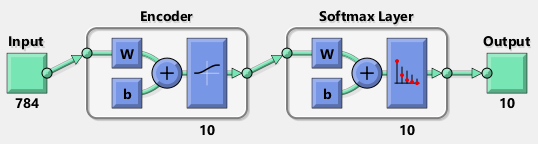
\includegraphics[scale=0.5]{image_9}
\end{flushleft}
\end{par}


\label{H_32BFAA67}
\matlabheadingtwo{3.3.1 Classifier with 30 Features}

\begin{matlabcode}
stackednet_30 = stack(autoenc_30, classifier_layer_30);
view(stackednet_30);
\end{matlabcode}

\begin{par}
\begin{flushleft}
\centering
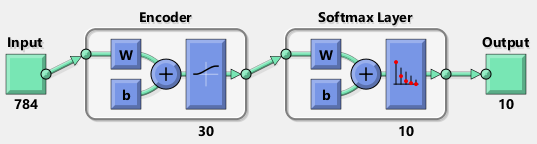
\includegraphics[scale=0.5]{image_10}
\end{flushleft}
\end{par}


\label{H_FD3D3197}
\matlabheadingtwo{3.3.1 Classifier with 60 Features}

\begin{matlabcode}
stackednet_60 = stack(autoenc_60, classifier_layer_60);
view(stackednet_60);
\end{matlabcode}

\begin{par}
\begin{flushleft}
\centering
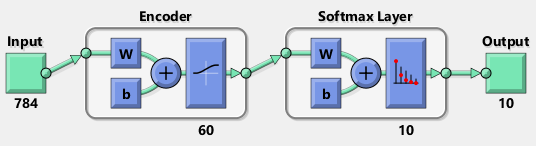
\includegraphics[scale=0.5]{image_11}
\end{flushleft}
\end{par}


\label{H_2810DB9B}
\matlabheading{3.4 Classification Performance Versus Number of Hidden Units}

\begin{par}
\begin{flushleft}
Here we have investigated the performance of the classifiers (constructed above) on the whole test set of the MNIST dataset.
\end{flushleft}
\end{par}

\begin{matlabcode}
predicted_labels_5 = stackednet_5(train_images_reshaped);
predicted_labels_10 = stackednet_10(train_images_reshaped);
predicted_labels_30 = stackednet_30(train_images_reshaped);
predicted_labels_60 = stackednet_60(train_images_reshaped);

performance_5 = 1 - confusion(test_labels_one_hot_encoded, predicted_labels_5);
performance_10 = 1 - confusion(test_labels_one_hot_encoded, predicted_labels_10);
performance_30 = 1 - confusion(test_labels_one_hot_encoded, predicted_labels_30);
performance_60 = 1 - confusion(test_labels_one_hot_encoded, predicted_labels_60);

performance = [performance_5 performance_10 performance_30 performance_60] * 100;
num_of_hidden_layers = [5 10 30 60];
plot(num_of_hidden_layers, performance, 'Marker', "o", 'LineStyle',"--", 'LineWidth', 2);
xlim([0 65]);
ylim([0 100]);
grid on;
xticks(num_of_hidden_layers);
ylabel('Percentage of Correct Prediction (%)');
xlabel('# of Hidden Units');
title('Performance on Test Dataset vs. Number of Hidden Units');
\end{matlabcode}
\begin{center}
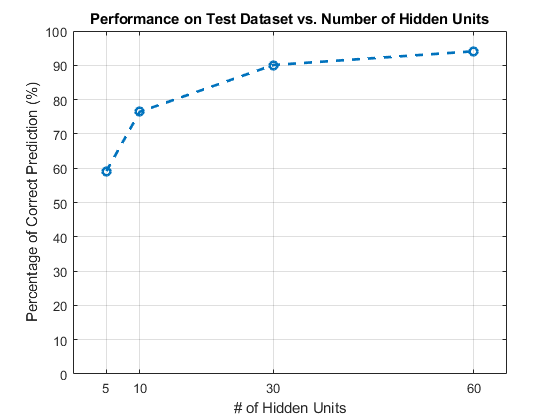
\includegraphics[width=\maxwidth{56.196688409433015em}]{figure_9.png}
\end{center}
\pagebreak

\label{T_76FF2B24}
\matlabtitle{4. Confusion Matrices}

\begin{par}
\begin{flushleft}
Confusion matrices for every classifier of the previous part is plotted in this section.
\end{flushleft}
\end{par}

\label{H_F6446B0C}
\matlabheading{4.1 Confusion Matrix for 5 Unit Classifier }

\begin{matlabcode}
plotconfusion(iCategorical(test_labels_one_hot_encoded), iCategorical(predicted_labels_5));
\end{matlabcode}
\begin{center}
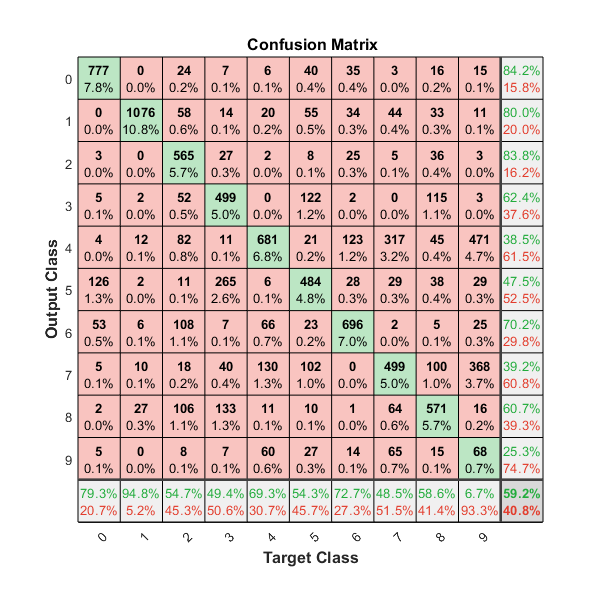
\includegraphics[width=\maxwidth{60.210737581535376em}]{figure_10.png}
\end{center}
\pagebreak

\label{H_A78337F0}
\matlabheading{4.2 Confusion Matrix for 10 Unit Classifier }

\begin{matlabcode}
plotconfusion(iCategorical(test_labels_one_hot_encoded), iCategorical(predicted_labels_10));
\end{matlabcode}
\begin{center}
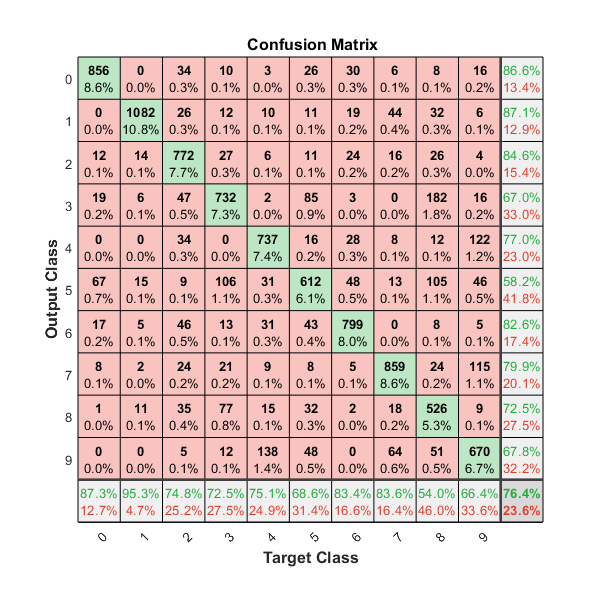
\includegraphics[width=\maxwidth{60.210737581535376em}]{figure_11.png}
\end{center}
\pagebreak

\label{H_0BF8770F}
\matlabheading{4.3 Confusion Matrix for 30 Unit Classifier }

\begin{matlabcode}
plotconfusion(iCategorical(test_labels_one_hot_encoded), iCategorical(predicted_labels_30));
\end{matlabcode}
\begin{center}
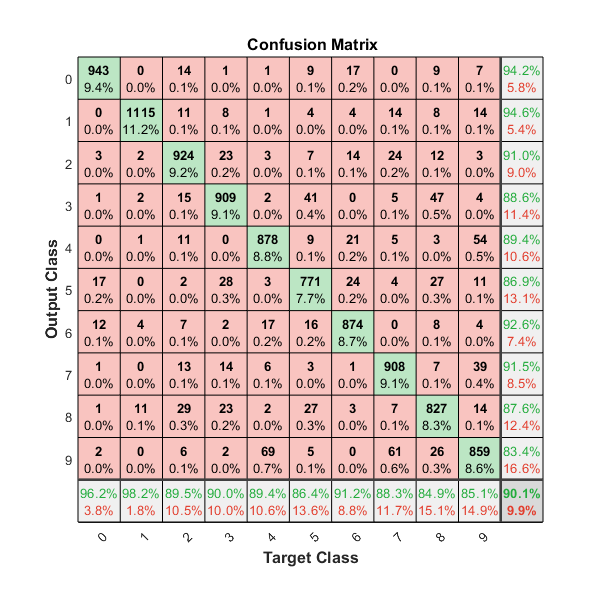
\includegraphics[width=\maxwidth{60.210737581535376em}]{figure_12.png}
\end{center}
\pagebreak

\label{H_93325639}
\matlabheading{4.4 Confusion Matrix for 60 Unit Classifier }

\begin{matlabcode}
plotconfusion(iCategorical(test_labels_one_hot_encoded), iCategorical(predicted_labels_60));
\end{matlabcode}
\begin{center}
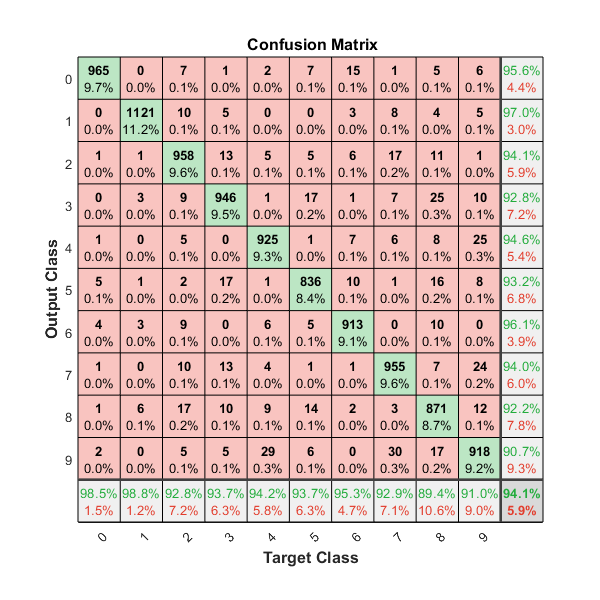
\includegraphics[width=\maxwidth{60.210737581535376em}]{figure_13.png}
\end{center}
\pagebreak

\label{T_11BC320C}
\matlabtitle{5. Encoder Weights Comparing to PCA Eigenvectors and K-means Centroids}

\begin{par}
\begin{flushleft}
First we repeat plotting the weights of autoencoders with 10 and 30 hidden units.
\end{flushleft}
\end{par}

\begin{matlabcode}
iMontage(autoenc_10.EncoderWeights');
\end{matlabcode}
\begin{center}
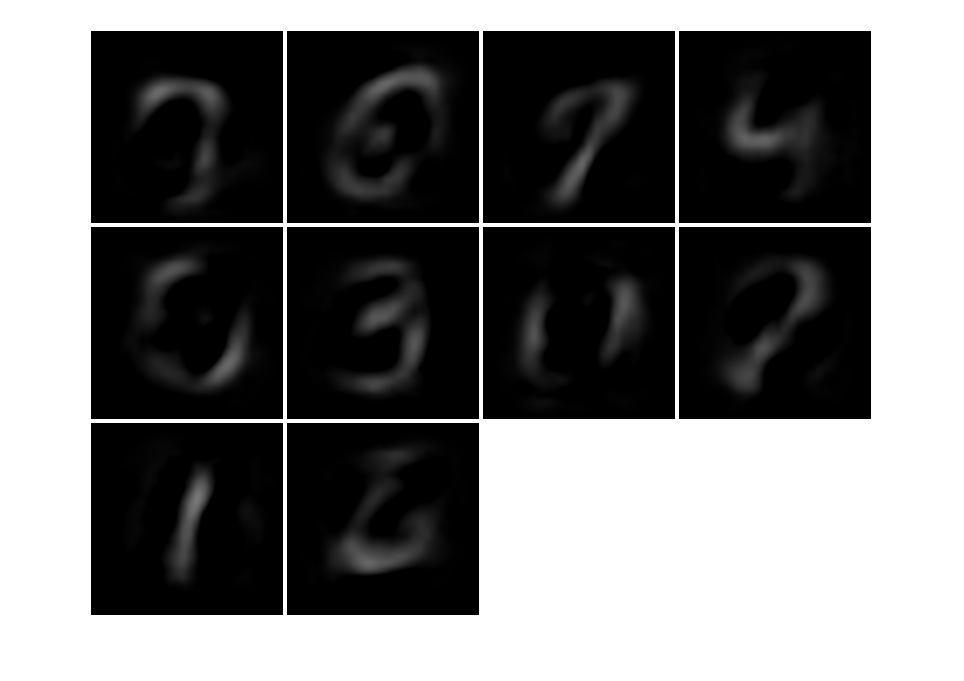
\includegraphics[scale=0.3]{figure_14.png}
\end{center}
\begin{matlabcode}
iMontage(autoenc_30.EncoderWeights');
\end{matlabcode}
\begin{center}
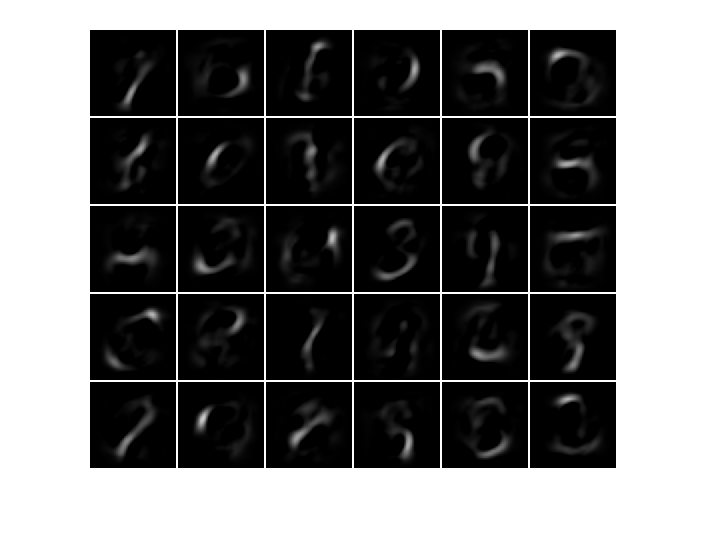
\includegraphics[scale=0.4]{figure_15.png}
\end{center}

\begin{par}
\begin{flushleft}
It can be seen from the figures above that:
\end{flushleft}
\end{par}

\begin{itemize}
\setlength{\itemsep}{-1ex}
   \item{\begin{flushleft} Some wieghts of the autoencoder with 10 hidden units are actually a replica of a handwritten image, for example digits 0, 1, 3, 4, 6 and 7 could be seen in them. \end{flushleft}}
   \vspace{3pt}
   \item{\begin{flushleft} Autoencoder with 30 hidden units will be more precise in classifying images because every hidden node will be fired if a small pattern be found in the input image. The weights are not similar to  a whole digit (as it was for autoencoder with 10 hidden units), but a portion of them are able to detect and reconstruct an image more precisely.  \end{flushleft}}
\end{itemize}

\begin{par}
\begin{flushleft}
The first 10 PCA eigenvectors from HW\#3 is plotted in figure below:
\end{flushleft}
\end{par}

\begin{par}
\begin{flushleft}
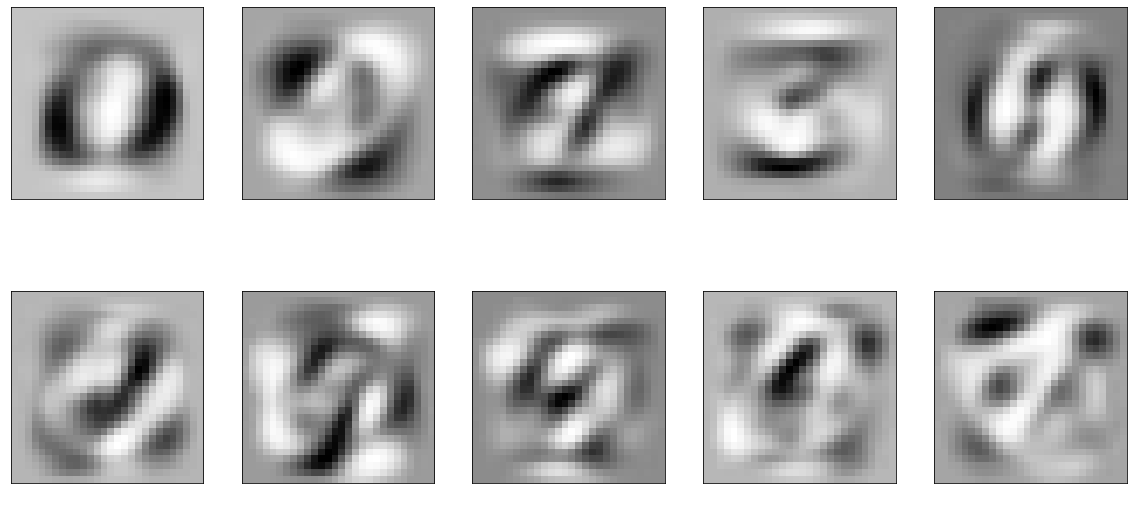
\includegraphics[width=\maxwidth{52.88509784244857em}]{image_12}
\end{flushleft}
\end{par}

\begin{par}
\begin{flushleft}
Here we can see a trace of digits 0, 1, 3 and 6 in the PCA eigenvectors.
\end{flushleft}
\end{par}


\vspace{1em}
\begin{par}
\begin{flushleft}
10 K-means centroids from HW\#4 are plotted below:
\end{flushleft}
\end{par}

\begin{par}
\begin{flushleft}
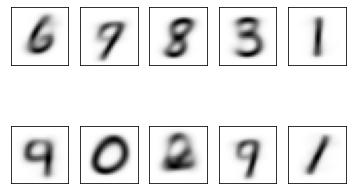
\includegraphics[width=\maxwidth{54.189663823381835em}]{image_13}
\end{flushleft}
\end{par}

\begin{par}
\begin{flushleft}
These centroids are much more like handwritten digits because they are constructed actually from averaging over the clusters of digits.
\end{flushleft}
\end{par}

\begin{par}
\begin{flushleft}
It is worth mentioning that PCA and K-means are linear dimensionality reduction algorithms however, autoencoders try to encode the images with neurons which have nonlinear activation functions. 
\end{flushleft}
\end{par}
\pagebreak

\label{T_F8AA430C}
\matlabtitle{Appendix}

\label{H_64B544B3}
\matlabheading{A.1 Saving Workspace Variables for Future Use }

\begin{matlabcode}
save('HW9_code_workspace.mat')
\end{matlabcode}


\label{H_430FCF21}
\matlabheading{A.2 Defiition of Auxiliary Functions}

\begin{matlabcode}
function downloadMNIST(mnist_train_image, mnist_train_label, mnist_test_image, mnist_test_label)

if exist('train-images-idx3-ubyte','file') ~= 2
    disp('Downloading MNIST dataset...');
    websave([mnist_train_image,'.gz'],...
        ['http://yann.lecun.com/exdb/mnist/', ...
        mnist_train_image, '.gz']);
    websave([mnist_train_label,'.gz'],...
        ['http://yann.lecun.com/exdb/mnist/', ...
        mnist_train_label, '.gz']);
    websave([mnist_test_image,'.gz'],...
        ['http://yann.lecun.com/exdb/mnist/', ...
        mnist_test_image, '.gz']);
    websave([mnist_test_label,'.gz'],...
        ['http://yann.lecun.com/exdb/mnist/', ...
        mnist_test_label, '.gz']);
    disp('MNIST dataset downloded.');
    
    disp('Unzipping started...');
    gunzip([mnist_train_image, '.gz'])
    gunzip([mnist_train_label, '.gz'])
    gunzip([mnist_test_image, '.gz'])
    gunzip([mnist_test_label, '.gz'])
    delete([mnist_train_image, '.gz'])
    delete([mnist_train_label, '.gz'])
    delete([mnist_test_image, '.gz'])
    delete([mnist_test_label, '.gz'])
    disp('Unzipping completed.');
else
    disp('MNIST dataset already downloaded.')
end

end

function [imgs, labels] = readMNIST(imgFile, labelFile, num_of_digits_to_read)

fileID = fopen(imgFile, 'r', 'b');
header = fread(fileID, 1, 'int32');

if header ~= 2051
    error('Invalid image file header');
end

count = fread(fileID, 1, 'int32');

if count < num_of_digits_to_read
    error('Trying to read too many digits');
end

rows_num = fread(fileID, 1, 'int32');
cols_num = fread(fileID, 1, 'int32');

imgs = zeros([rows_num cols_num num_of_digits_to_read]);

for i = 1:num_of_digits_to_read
    for row = 1:rows_num
        imgs(row, :, i) = fread(fileID, cols_num, 'uint8');
    end
end

fclose(fileID);

fileID = fopen(labelFile, 'r', 'b');
header = fread(fileID, 1, 'int32');

if header ~= 2049
    error('Invalid label file header');
end

count = fread(fileID, 1, 'int32');

if count < num_of_digits_to_read
    error('Trying to read too many digits');
end

labels = fread(fileID, num_of_digits_to_read, 'uint8');

fclose(fileID);

imgs = double(imgs)./255.0;

end

function iMontage(images)
montage(reshape(images, [28 28 size(images, 2)]), 'BackgroundColor', 'white', 'BorderSize', [2 2]);
end

function display_original_images_vs_reconstructed(original_images, reconstructed_images)
figure('Position', [100, 100, 1000, 500]);
subplot(1, 2, 1);
iMontage(original_images);
title('Original Images');
hold on;
subplot(1, 2, 2);
iMontage(reconstructed_images);
title('Reconstructed Images')
hold off
end

function categorized_label = iCategorical(on_hot_encoded_label)
[ind, ~]= vec2ind(on_hot_encoded_label);
categorized_label = categorical(ind', 1:10, {'0' '1' '2' '3' '4' '5' '6' '7' '8' '9'});
end
\end{matlabcode}

\end{document}
